\documentclass[a4paper,12pt]{article}

\usepackage{rotating}
\usepackage[top=1.25in, bottom=1.25in, left=1.25in, right=1.25in]{geometry}
\usepackage{graphicx}
\usepackage[numbers,square,sort&compress]{natbib}
\usepackage{setspace}
\usepackage[cdot,mediumqspace,]{SIunits}
\usepackage{caption}
\usepackage{subcaption}
\usepackage{mathtools}
\usepackage{authblk}
\usepackage{float}
\usepackage{wrapfig}
\renewcommand{\thesubsection}{\thesection.\alph{subsection}}
\providecommand{\e}[1]{\ensuremath{\times 10^{#1}}}
\newcommand*\lap{\mathop{}\!\mathbin\bigtriangleup}

\begin{document}
\onehalfspacing
\title{Special Functions and Solving the Heat Equation for a Cold Cylinder}
\author{Natalie Price-Jones, 999091021}
\date{4 December 2014}
\affil{\small{natalie.price.jones@mail.utoronto.ca}}
\maketitle

\section{Physics Background}
%
%\begin{wrapfigure}{r}{0.3\textwidth}
%  \begin{center}
%    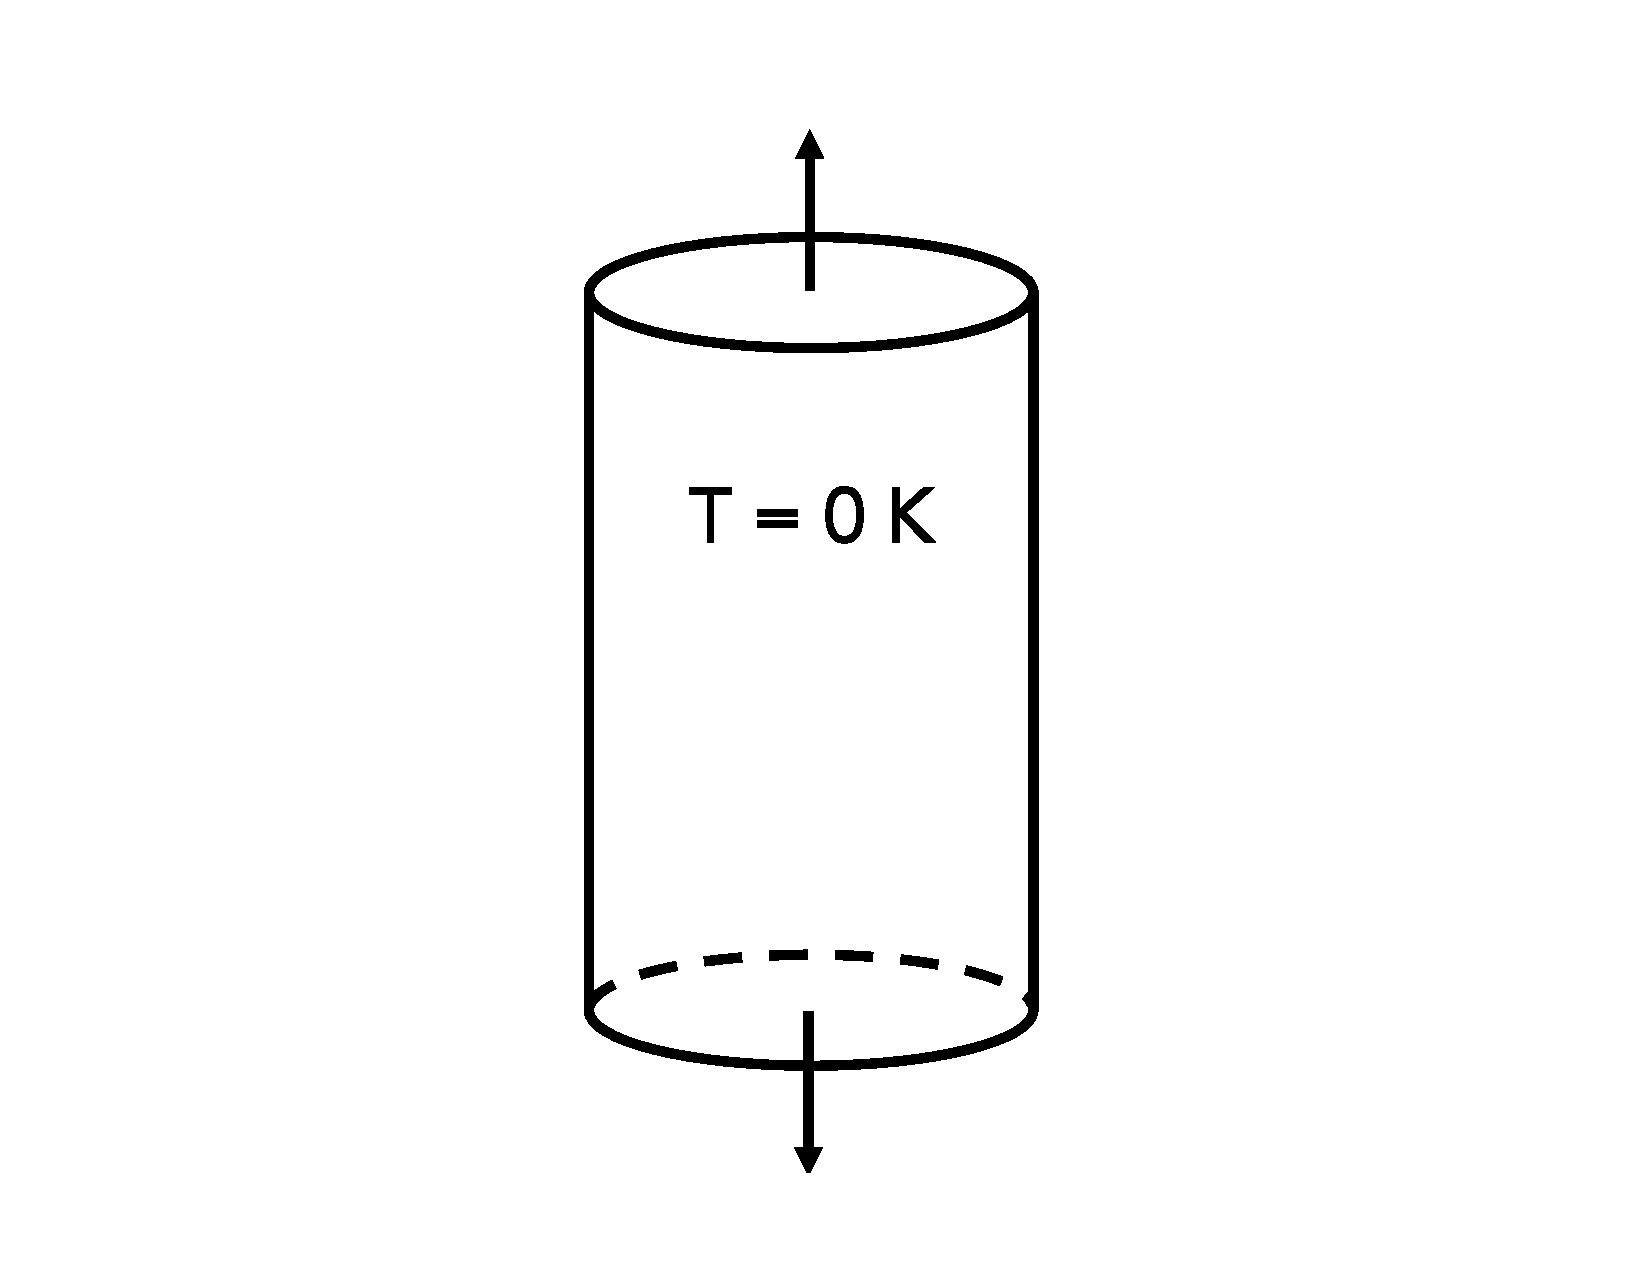
\includegraphics[width=0.28\textwidth]{coldcylinder}
%  \end{center}
%  \caption{}
%\label{fig:cyl}
%\end{wrapfigure}

In this lab, we will solve the heat equation ($\frac{\partial u}{\partial t} = c\lap u$ where $\lap$ is the Laplacian operator) for a solid cylinder. We start with a cylinder at some uniform temperature $T_0$. Then we hold the environment around the cylinder at a constant temperature $T = T_1 = 0 K$, where $T_0 > T_1 > 0K$. Common sense tells us that the cylinder will equilibrate with its surroundings, its temperature decreasing until it reaches uniform $T = 0K$. The temperature change over time and position is described by the heat equation. For simplicity, we will assume our cylinder has infinite length and radius $R$. This reduces the problem to a single dimension, the radial coordinate $s$ (since our initial temperature profile now has only radial dependence). So we wish to solve the following PDE:

\begin{displaymath}
   \left\{
   	\begin{equation}
     \begin{array}{c}
     \frac{\partial u}{\partial t} = \frac{c}{s}\frac{\partial}{\partial s}\left(s\frac{\partial u}{\partial s}\right)\: : \: s \leq R,\, t > 0\\
     u(t = 0, s)  = T_0\\
     u(t,s = R) = 0
     \end{array}
     \label{eqn:pde}
     \end{equation}
   \right.
\end{displaymath} 
%
where $u(t,s)$ is the temperature as a function of time $t$ and distance from the centre of the cylinder $s$ and $c$ in our case is thermal diffusivity. We have learned a lot of techniques to numerically solve PDEs, but it turns out that Equation \ref{eqn:pde} can be solved analytically (sort of). If we employ separation of variables by assuming $u(t,s) = T(t)S(s)$, we can reduce it to two ODEs,

\begin{eqnarray}
\frac{1}{c T(t)}\frac{dT(t)}{dt} &=& -\lambda^2\nonumber\\
\frac{1}{S(s)}\frac{d^2 S(s)}{ds^2} + \frac{1}{s\,S(s)}\frac{dS(s)}{ds} &=& -\lambda^2
\label{eqn:ode} 
\end{eqnarray} 

Here, $T$ is a function of only time whose product with $S$ constructs $u$, not the temperature itself. $-\lambda^2$ is an eigenvalue. The solution for $T(t)$ is simply an exponential, but the solution to Equation \ref{eqn:ode} is not immediately obvious if you haven't seen it before. If we make a substitution $z = \lambda s$ and rearrange slightly, we see that Equation \ref{eqn:ode} is a form of Bessel's differential equation of order zero:

\begin{equation}
0 = \frac{d^2S(z)}{dz^2} + \frac{1}{z}\frac{dS(z)}{dz} + S(z)\nonumber
\end{equation}

The solutions to this equation are order zero Bessel functions of the first ($J_0(z)$) and second ($Y_0(z)$) kind (see Figure \ref{fig:bes}). So our final solution $S(z)$ should be a linear combination of these two functions.

\begin{figure}[H]
\centering
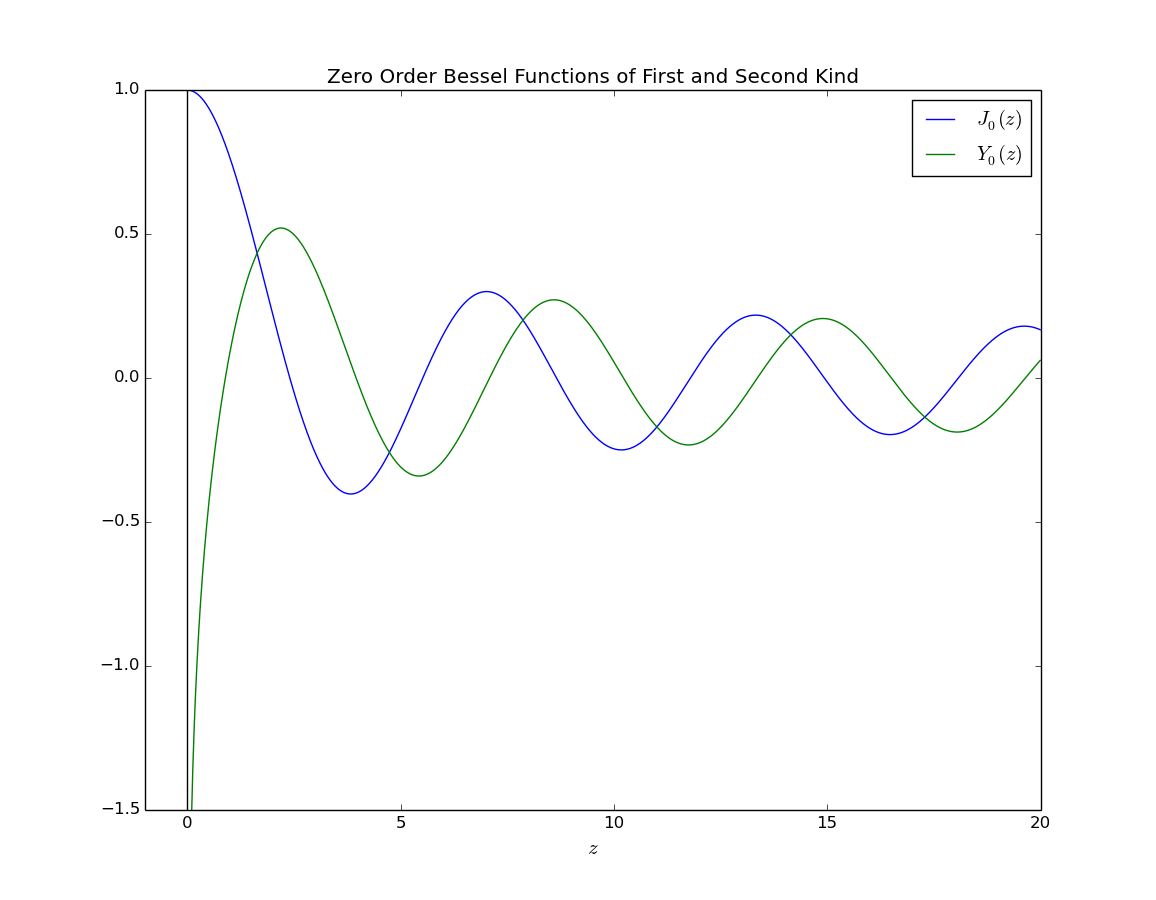
\includegraphics[width = \linewidth]{bessel.png}
\caption{Zero order Bessel functions, created using scipy.special module.}
\label{fig:bes}
\end{figure}

We can see in Figure \ref{fig:bes} that $Y_0(z) \rightarrow -\infty$ as $z\rightarrow 0$. But both the initial and boundary conditions imply $S(s)$ must be finite as $s\rightarrow 0$, and since $z\propto s$, we need $S(z)$ finite as $z\rightarrow 0$. For the purposes of solving Equation \ref{eqn:bes}, we discard the $Y_0(z)$ solution. The solution for $S(s)$ will be a linear combination of $J_0(\lambda s)$ for different $\lambda$ eigenvalues. Using the boundary condition from Equation \ref{eqn:pde} and the orthogonality properties of the zero order Bessel functions, it is possible to determine a closed form solution to the PDE we have set out to solve. This derivation is shown in Appendix \ref{app:deriv}, but the result is given below:

\begin{equation}
u(t,s) = 2 T_0\sum_{m = 1}^{\infty}\frac{e^{-\lambda_m^2 c\,t}}{\lambda_m R}\frac{J_0(\lambda_m s)}{J_1(\lambda_m R)},
\label{eqn:final}
\end{equation}
%
where $\lambda_m$ is chosen so $J_0(\lambda_m R) = 0$.

Equation \ref{eqn:final} isn't in a form we really want when we try to code the result. For one thing, its an infinite series - we may be able to approximate it with sufficient numbers of terms but it would be impossible to find an exact solution. Even worse, the result depends on these Bessel functions, but I've not yet said what these are. In fact these function are very important to many other kinds of calculations, so much so that they are included in the scipy.special module as callable functions.

The Bessel functions have multiple definitions. Since we are concerned with functions of integer order, we will consider the following two:

\begin{eqnarray}
J_n(x) &=& \sum_{k=0}^{\infty}\frac{(-1)^k}{k!(k+n)!}\left(\frac{x}{2}\right)^{2k+n}\label{eqn:bessum}\\
\mathrm{and}\:\: J_n(x) &=& \frac{1}{\pi}\int_{0}^{\pi}\cos(n\tau - x\sin(\tau))d\tau
\label{eqn:besint}
\end{eqnarray}

\section{Computational Background}

\subsection{Memoization}

Memoization is a very fancy term for a relatively simple idea: taking advantage of a computer's memory rather than its processor. Imagine you have many iterations of a complicated calculation, and each new iteration depends on the previous one. Obviously you would want to save the results of your calcuation so you can use previous results in your current iterations without recalculating them. In this course, we have used lists and arrays to track these sorts of numbers. The memoization tool of choice is usually dictionaries, as this allows you to link an independent variable to the results you want to store. This means you don't need to know anything about the list - just the appropriate independent variable to call your result.

But this isn't so different from what we've already done, storing the results of various iterations in lists. We can take the advantage a step further by saving our results, then calling them in when we need to make further calcuations.

\subsection{Interpolation}

Another method to minimize time consuming calculation is interpolation. Suppose you want to know the value of a smooth function at many points, but computing the value of the function takes far too long to specifically evaluate it at every location. The obvious solution is to evaluate the function at only a few points, then use these values to infer what the function looks like everywhere else. There are a few caveats: as I've said, you need your function to be smooth and continuous. If your function isn't well behaved, you'll need a near infinite number of points to calculate its shape. And even when your function is smooth and continuous, you still to be sure that you are sampling the right number of points in order to truly describe the function.

\section{Lab Instructions}

For grading purposes, only hand in the following parts. Ensure codes are well commented and readable by an outsider.

\begin{itemize}
\item Q1: 
  \begin{itemize}
    \item Hand in the functions written for all three parts in a single file. 
    \item Make a table comparing the speed of each part's method. 
    \item State for each method what happens when 1000! is evaluated. 
    \item Provide short answers for parts b),c) and d).
  \end{itemize}

\item Q2: 
  \begin{itemize}
    \item Hand in your code for parts b) and d).
    \item Turn in plots for b) and c) with all curves for all three numbers of sum terms on the same plot. 
    \item Hand in a plot for part d) comparing your curve with the results of the scipy module. 
    \item Hand in a plot of part f). 
    \item Provide short answers for parts b),c) and e).
  \end{itemize}

\item Q3: 
  \begin{itemize}
    \item Hand in your code for part a) and the accuracy needed.
    \item Provide a short answer for part b)
  \end{itemize}

\item Q4:
  \begin{itemize}
    \item Hand in your code
    \item Hand in a snapshot of your animations at t = 0, 0.005,10 and 100.
    \item Provide a short answer to the question asked.
  \end{itemize}
\end{itemize}
\\
\textbf{Question 1:} One of the biggest challenges in computing Bessel functions using Equation \ref{eqn:bessum} lies in finding factorials effeciently. Python's built in math module provides a function to do this (math.factorial).\\
\textbf{a)} Write a recursive factorial function and compute factorials for 10,100,500. What happens when you try to find the factorial of 1000? How does the speed of the computation compare with using math.factorial?\\
\textbf{b)} A common way to approximate large factorials is to use Stirling's approximation, $\ln(n!) \approx n\ln(n) - n$. Can we compute factorial of 1000 with this? How does $\ln(1000!)$ compare with math.log(math.factorial(1000))? What about $\ln(1\e{5}!)$ compared with math.log(math.factorial($1\e{5}$))? Which computation takes longer?\\
\textbf{c)} Another technique that can be used to improve factorial computation is memoization, described in the Computational Background. Using memoization write a new recursive function that computes the a factorial. Use this new function, find the factorial (in order) of 1000, 10, 100, 500, 1000. What happened when you tried to evaluate 1000! each time?  With this in mind, explain one advantage and one disadvantage of this method of computing factorials. \\
\textbf{d)} Choose one of the three fuctions you developed to use in the remainder of the program and explain your choice.\\

\textbf{Question 2:} \\
\textbf{a)} Simplify Equations \ref{eqn:bessum} and \ref{eqn:besint} for the cases where $n = 0$ and $n = 1$.\\
\textbf{b)} Find $J_0(x)$ from $x$ = 0 to $x$ = 20 with step size 0.01 using Equation \ref{eqn:bessum} with 25 terms. Do the same for 50 and 75 terms. How does increasing the number of terms change your results? \\
\textbf{c)} What happens if you perform the same three evaluations as in part b) but change the upper bound of your x range to $x$ = 40? Why do we see this result? \\
\textbf{d)} Use one of the integration methods we developed in Labs 2 and 3 to evaluate Equation \ref{eqn:besint}. Do your results match those of the scipy module?\\
\textbf{e)} Based on the results of part b), choose either Equation \ref{eqn:bessum} or Equation \ref{eqn:besint} to use for the remainder of the lab and justify your selection.\\
\textbf{f)} Use your choice from c) to evaluate $J_1(x)$ on the same $x$ range as part b). \\

\textbf{Question 3:} A necessary component of Equation \ref{eqn:final} is knowing for which $\lambda_m$ $J_0(\lambda_m R) = 0$. Solving for eigenvalues $\lambda_m$ is equivalent to finding the zeros of the Bessel function and dividing them by $R$.\\
\textbf{a)} Use any of the zero-finding methods of Lab 4 to find the first five zeros of $J_0$. Use the $J_0$ you chose in question 2 part e). Compare your results with the output of scipy.special.jn\_zeros and adjust your accuracy until you get a match to 9 significant figures. What (approximate) accuracy was needed to reproduce scipy's result?\\
\textbf{b)} Although Bessel functions are not periodic, the location of their nth zero can be approximated using $\pi\left(n-1/4\right)$. Use this to approximate the location of the 5th, 50th and 500th zeros. Does your location for the 5th zero match what you found in part a)? Compare your result with scipy.special.jn\_zeros. For which n is this a good approximation?  \\

\textbf{Question 4:} We now have all the tools we need to construct Equation \ref{eqn:final}. Create a function that produces the temperature at given time and position with a set number of terms for the sum. Use initial cylinder temperature $T_0 = 50$, radius $R = 10$ and $c = 1.25$, all with arbitrary units. Now use your function to create an animation of your function as time goes from 0 to 100 in the arbitrary units of the problem. Can you explain the shape of the function at $t = 0$? Does the function behave as expected at time proceeds?

\appendix

\section{Deriving a Closed Form Solution to the Heat Equation}
\label{app:deriv}

We have $S(z) = S(\lambda s) \sim J_0(\lambda s)$. The boundary condition in Equation \ref{eqn:pde} requires that our choice of $\lambda$ must satisfy $J_0(\lambda R) = 0$. However we saw in Figure \ref{fig:bes} that Bessel functions are oscillatory, and so there are infinite choices for $\lambda$ that satisfy this requirement. If we denote them $\lambda_m$ then we know $u(t,s)$ is a linear combination over all possible eigenvalues.

\begin{eqnarray}
S_m(s) &=& c_m J_0(\lambda_m s)\nonumber\\
\mathrm{and}\:\: T_m(t) &=& T_m(0)e^{-\lambda_m^2 c\,t}\nonumber\\
\implies u(t,s) &=& \sum_{m=1}^{\infty}a_m e^{-\lambda_m^2 c\,t} J_0(\lambda_m s)\nonumber\\
\mathrm{since}\:\: u_m(t,s) &=& S_m(s)T_m(t)\:\:\mathrm{and}\:\: u(t,s) = \sum_{m=1}^{\infty}u_m(t,s)\nonumber 
\end{eqnarray}

Our $\lambda_m$ are implicitly defined by $J_0(\lambda_m R) = 0$, so we are left with determining the coefficients $a_m$.

With this in mind, note the orthogonality property of zero order Bessel functions of the first kind: 

\begin{equation}
\int_{0}^{R}s\,J_0(\lambda_m s)J_0(\lambda_n s)ds = \delta_{mn}\frac{R^2}{2}J_1^2(\lambda_m R)
\label{eqn:ortho}
\end{equation}
%
where we have introduced the first order Bessel function of the first kind $J_1$. We will also need another property of Bessel functions:
\begin{equation}
\int_{0}^{x} x'J_0(x')dx' = xJ_1(x).
\label{eqn:int}
\end{equation} 

This is easily verified by substituting Equation \ref{eqn:bessum} in for $J_0$ and $J_1$.

We know our solution must satisfy $u(t=0,s) = T_0$, so we have:

\begin{equation}
T_0 = \sum_{m=1}^{\infty}a_m J_0(\lambda_m s)\nonumber
\end{equation}

If we multiply this expression on each side by $s\,J_0(\lambda_n s)$ and integrate, we can exploit Equation \ref{eqn:ortho} to isolate for $a_m$.

\begin{eqnarray}
a_m &=& \frac{2}{R^2 J_1^2(\lambda_m R)}\int_{0}^{R}T_0 s\,J_0(\lambda_m s)ds\nonumber\\
a_m &=& \frac{2}{R^2 J_1^2(\lambda_m R)} \frac{T_0 R\, J_1(\lambda_m R)}{\lambda_m}\nonumber\\
a_m &=& \frac{2 T_0}{\lambda_m R\, J_1(\lambda_m R)}\nonumber
\end{eqnarray}
%
where we have used Equation \ref{eqn:int} to go from the first to the second step.

Thus we find that:

\begin{eqnarray}
u(t,s) = \sum_{m=1}^{\infty}\frac{2 T_0}{\lambda_m R\, J_1(\lambda_m R)} e^{-\lambda_m^2 c\,t} J_0(\lambda_m s),\nonumber
\end{eqnarray}
%
which matches Equation \ref{eqn:final} above.
\end{document}
